\documentclass[%reprint,
%preprint, 
11pt,
amsmath, amssymb,
aps,
pra
]{revtex4-2}

\usepackage{bm}
\usepackage{dcolumn}
\usepackage{blindtext}
\usepackage{parskip}
\usepackage{graphicx}
\usepackage{subcaption}
\usepackage[en-US]{datetime2}
\usepackage{amsmath}
\usepackage{tabularx}

%\usepackage[none]{hyphenat}
\hyphenpenalty=10000
\hbadness=10000

\renewcommand{\thesection}{\arabic{section}}
\renewcommand{\thesubsection}{\thesection.\arabic{subsection}}
\renewcommand{\thesubsubsection}{\thesubsection.\arabic{subsubsection}}

\makeatletter
\def\Dated@name{Submitted: }
\makeatother

\newcommand{\threeImageSpacing}{0.25\textwidth}

\begin{document}

\title{Collective Motion: An investigation into the behaviours seen in nature}
\author{Dylan Scott}
\affiliation{Durham University, Department of Physics}
\DTMlangsetup{showdayofmonth=false}
\date{\today}


\begin{abstract}
In this paper, I investigate the nature of collective motion by studying and recreating more and more complex models
and making observations about fundamental parameters. In the single species models I measure the instability and transition
into disordered motion that occurs as the magnitude of the randomness in the movement is increased. Later, with the two species
models that focus on predator and prey type systems, I investigate the lifetime of the prey species as I tweak around the fundamental
starting parameters for each system. 
\end{abstract}

\maketitle

%\newpage

\tableofcontents
\section{Introduction}
The concept of collective motion covers a wide range of behaviours observed in nature. 
These behaviours include the coordinated flocking of birds, the fluid-like movements of schools of fish, 
the swarming of insects, and other such behaviours. It also includes the sudden disruption of such patterns, reducing
the ordered structure of a flock of starlings into a chaotic fluttering mess in the presence of a predatory species, for example.
Overall, collective motion can be considered as the coordination of a large group due to very simple rules followed
by each individual. 

As a research field, it has been discovered that collective motion may be applied in areas outside of 
ecological systems. Certain physical and chemical systems contain the presence of "self-propelled particles" which may
act in similar nature to the macroscopic animals described previously. For example, recent studies have examined 
things such as water condensation droplets \cite{lin2023emergent} and fermionic gases \cite{wang2023viscous}.
Given the vast amount of diverse situations in which the fundamental principles of collective motion apply, 
it is of interest that this field be studied. Grasping the underlying concepts may allow for a better understanding
of physical and chemical systems, and could also pave the way for future technological advancements. At present, there
have already been many studies investigating the applications of collective motion in autonomous drone flocks
\cite{verdoucq2022bio,zhao2018self,albani2022distributed}. These studies highlight the potential for practical 
implementations, where machines are capable of mirroring the coordination and collective behaviours observed in various
ecosystems.

As interesting as it would be to explore possible avenues for practical applications, the goal of this report will be
to provide an exploration of the concept of collective motion.
 I will cover the details of collective motion
as described in other research papers and articles and in addition will also be including my findings in the subject.
I will review several models constructed from previous reports and articles, recreate, and then test them. 
% In addition,
% I've replicated one of the basic models that will be highlighted in this report and reproduced similar datasets. 
% I should also mention that any model presented in this paper is one that has been presented in a past study on collective motion
% and then replicated and tested by myself, with no input from any of the original creators of these models.

\subsection{Basics of Collective Motion}

Collective motion is the name for the appearance of coherent behaviours or ordered movements from a group of individual units. 
The underlying principle is that each body may only follow a few simple rules, but this can result in the group performing
a range of complex movements. In general, collective motion normally occurs within a system when the units follow 
simple baseline rules: 
\begin{itemize}
    \item They are rather similar
    \item Move with near constant absolute velocity whilst capable of changing direction
    \item Interact within a specific interaction range and change direction based on its surrounding units
    \item Are subject to a noise of varying magnitude when choosing their movement direction
\end{itemize}
These rules, as specified by Vicsek \cite{vicsek2012collective}, govern the base principles that apply to all 
systems exhibiting collective motion. 

\begin{figure}[t]
    \begin{subfigure}{0.45\textwidth}
        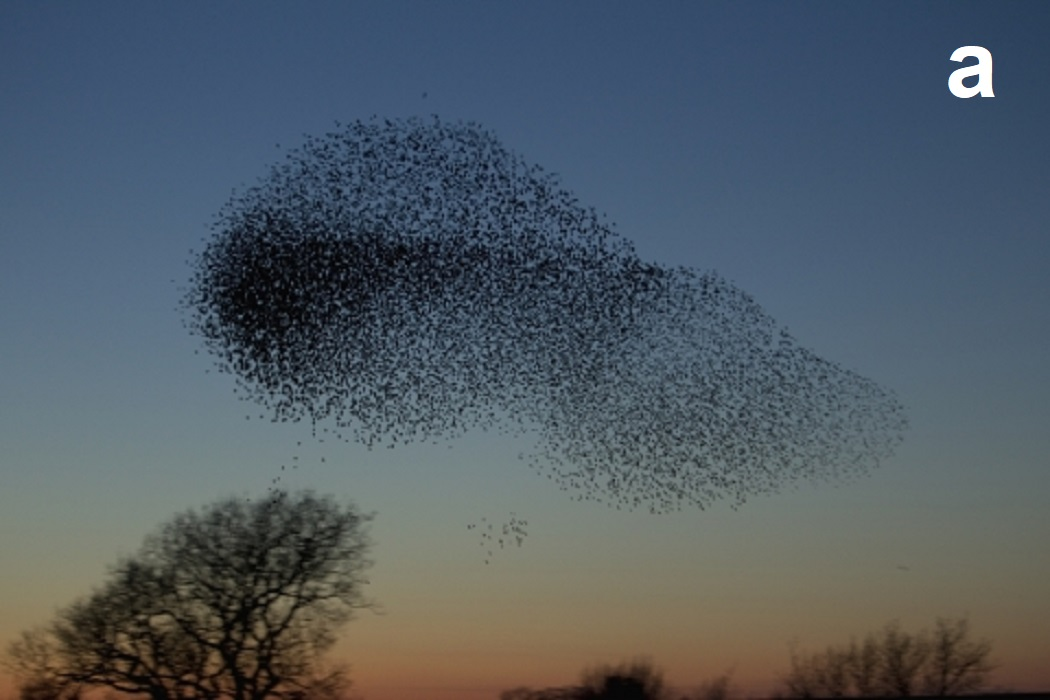
\includegraphics[width=\linewidth]{images/pictures/starling-flock.jpg}
    \end{subfigure}
    %\hspace{1cm}
    \begin{subfigure}{0.45\textwidth}
        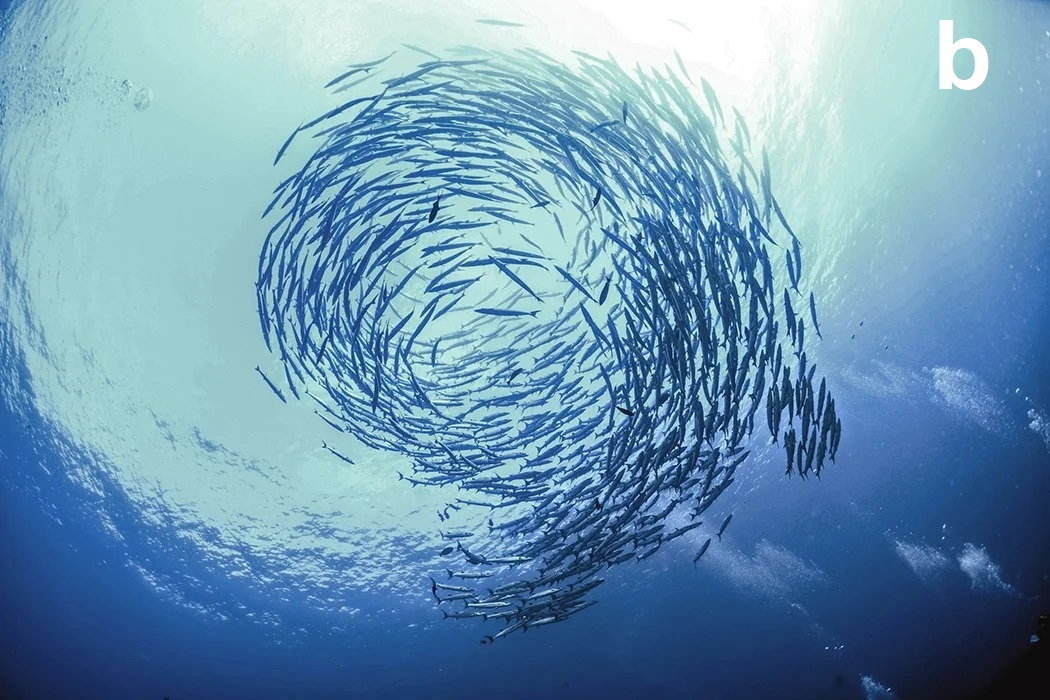
\includegraphics[width=\linewidth]{images/pictures/fish-school.jpg}
    \end{subfigure}
    \caption{A couple examples showcasing the complex collective motions that can be observed in nature.
    (a) a flock of birds
    (b) a vortex of schooling fish.}
    \label{fig:ExamplesOfCollectiveMotion}
\end{figure}

In nature, more complex motions and behaviours may arise as seen in Fig. \ref{fig:ExamplesOfCollectiveMotion}. The cause for 
such movements may be due to benefits to the species, such as protection from predators, or better efficiency in conserving stamina.





\section{Vicsek Model}
One of the first papers published on the subject was by Vicsek et al \cite{vicsek1995novel}. Their paper focused on the
complex cooperative behaviours that could be seen in particle systems going through a phase transition. They came up
with a simple model to replicate this behaviour.

\subsection{Vicsek Model Setup}
A set of \(N\) particles are placed within a 2D box of length \(L\) with periodic bounds. Initially, each particle has
a random starting position \(\mathbf{x}_i(t)\) and is set to move in a random direction \(\theta_i(t)\). The velocity \(\mathbf{v}_i(t)\)
of each particle is set to a constant speed \(|\mathbf{v}_i(t)| = v\). After every timestep \(\Delta t\) in the simulation, 
the positions and direction angles of the particles are adjusted in the following way:

\begin{align}
    \mathbf{x}_i(t + \Delta t) &= \mathbf{x}_i(t) + \mathbf{v}_i(t) \cdot \Delta t \\
    \theta_i(t + \Delta t) &= \left\langle \theta(t) \right\rangle _R + \Delta\theta 
\end{align}
The positions of the particles are updated in the usual way. The direction angle of each particle is calculated by taking the average
angle of all neighbouring particles within an interaction radius \(R\) and adding a \(\Delta\theta\) term which corresponds to a random perturbation of the angle.
The average angle may be calculated by 
\begin{figure}[t]
    \centering
    \begin{subfigure}{\threeImageSpacing}
        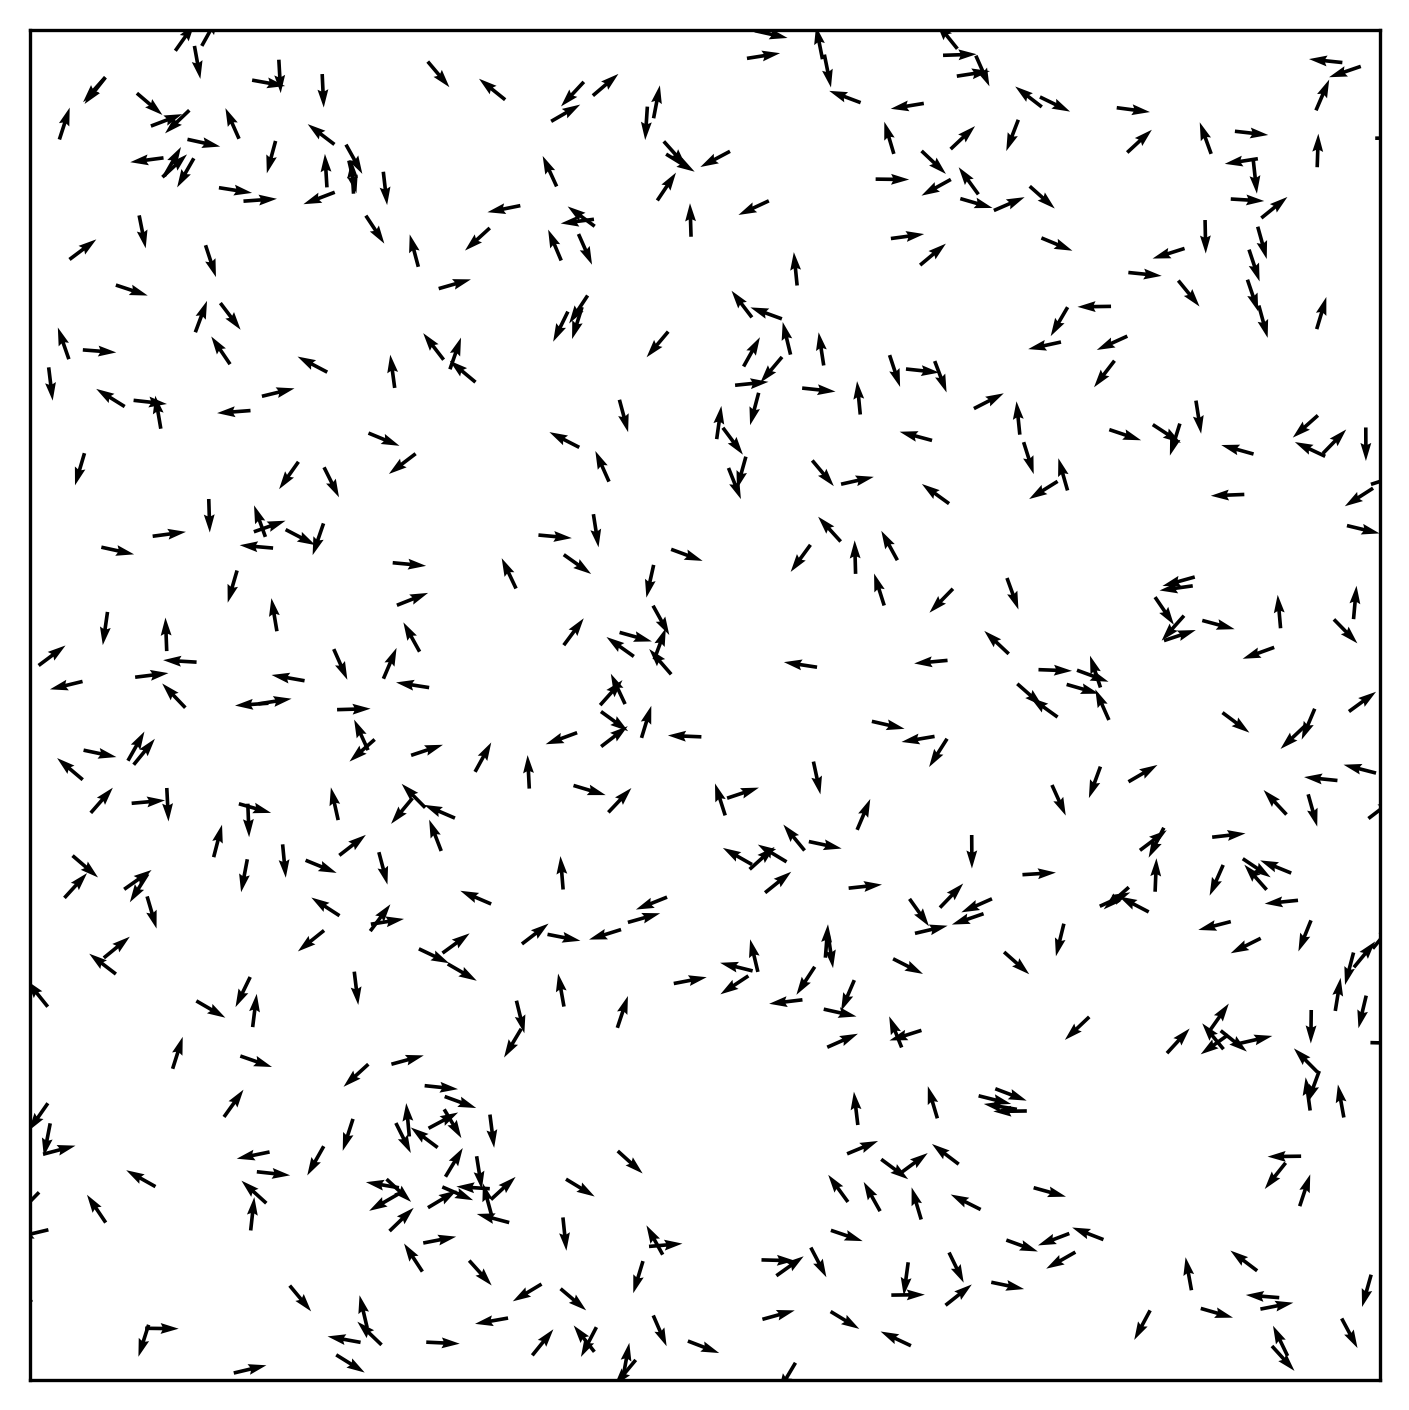
\includegraphics[width=\linewidth]{images/vicsek/VicsekZero.png}
    \end{subfigure}
    %\hfill
    \begin{subfigure}{\threeImageSpacing}
        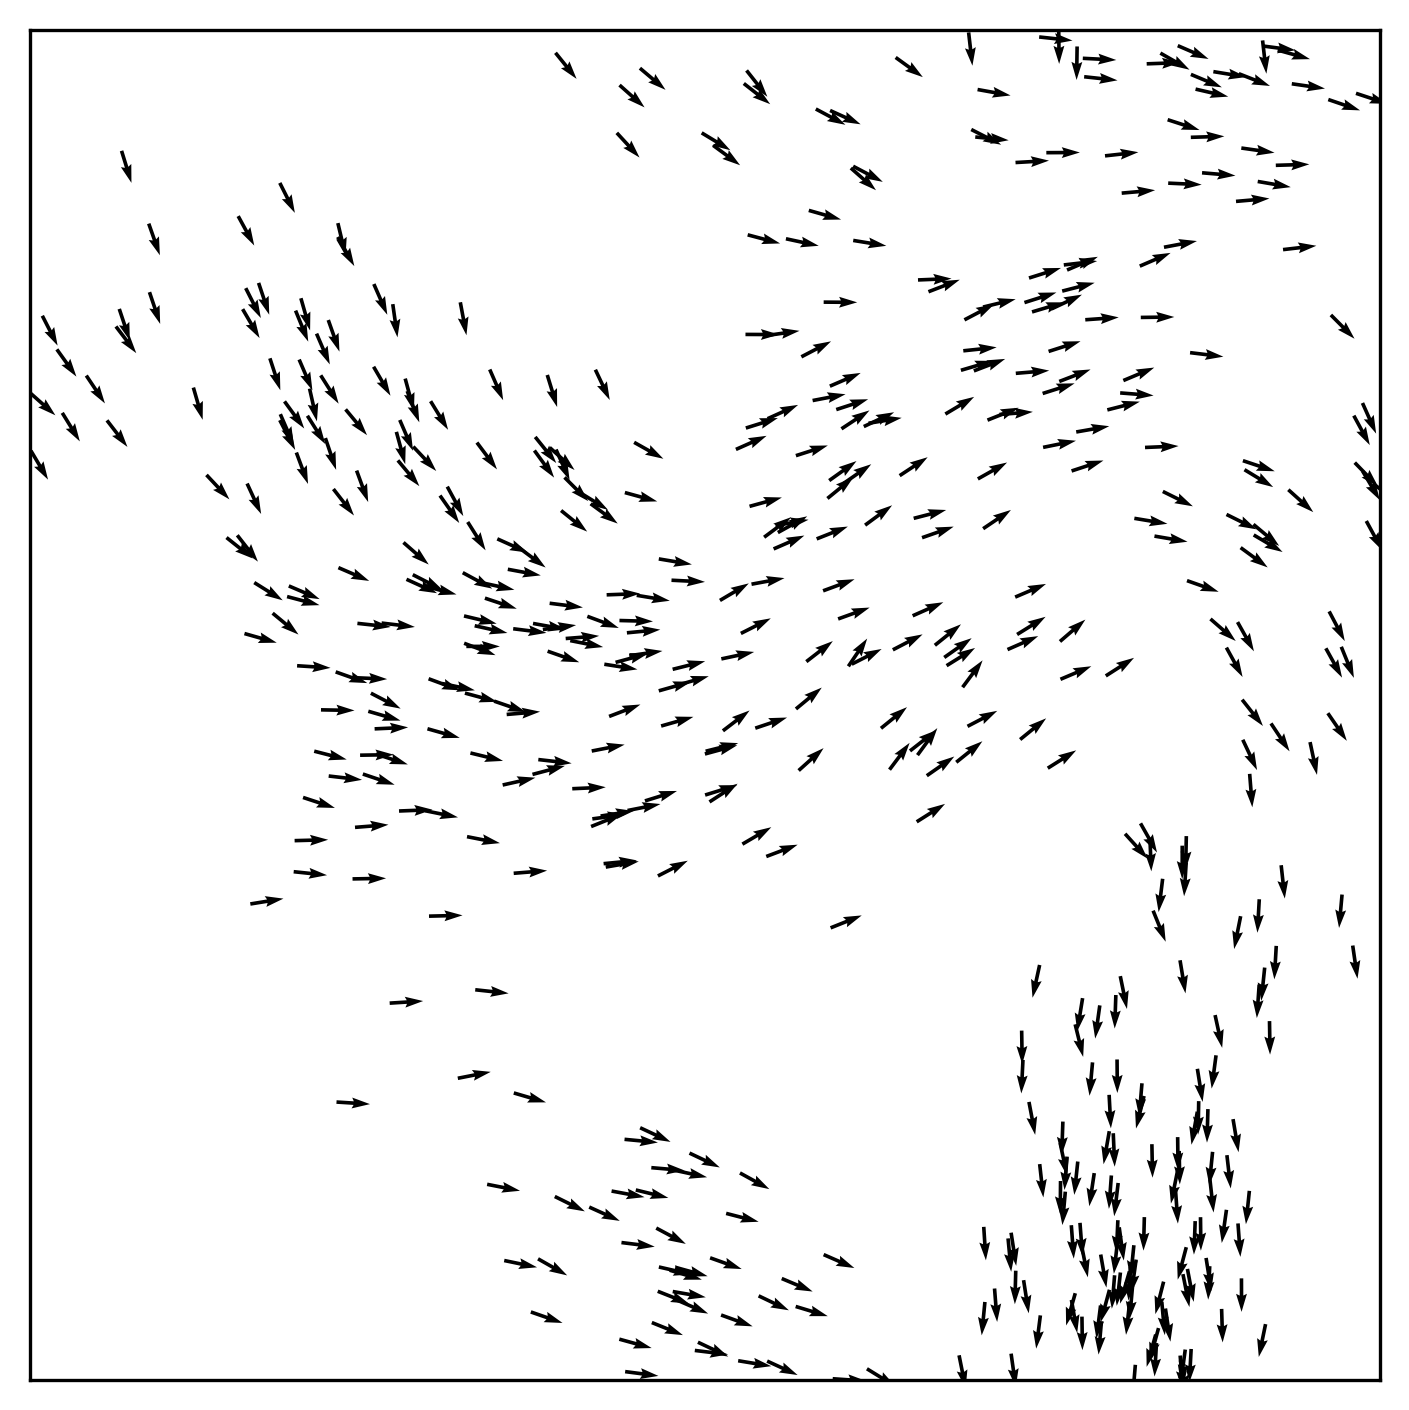
\includegraphics[width=\linewidth]{images/vicsek/Vicsek.png}
    \end{subfigure}
    %\hfill
    \begin{subfigure}{\threeImageSpacing}
        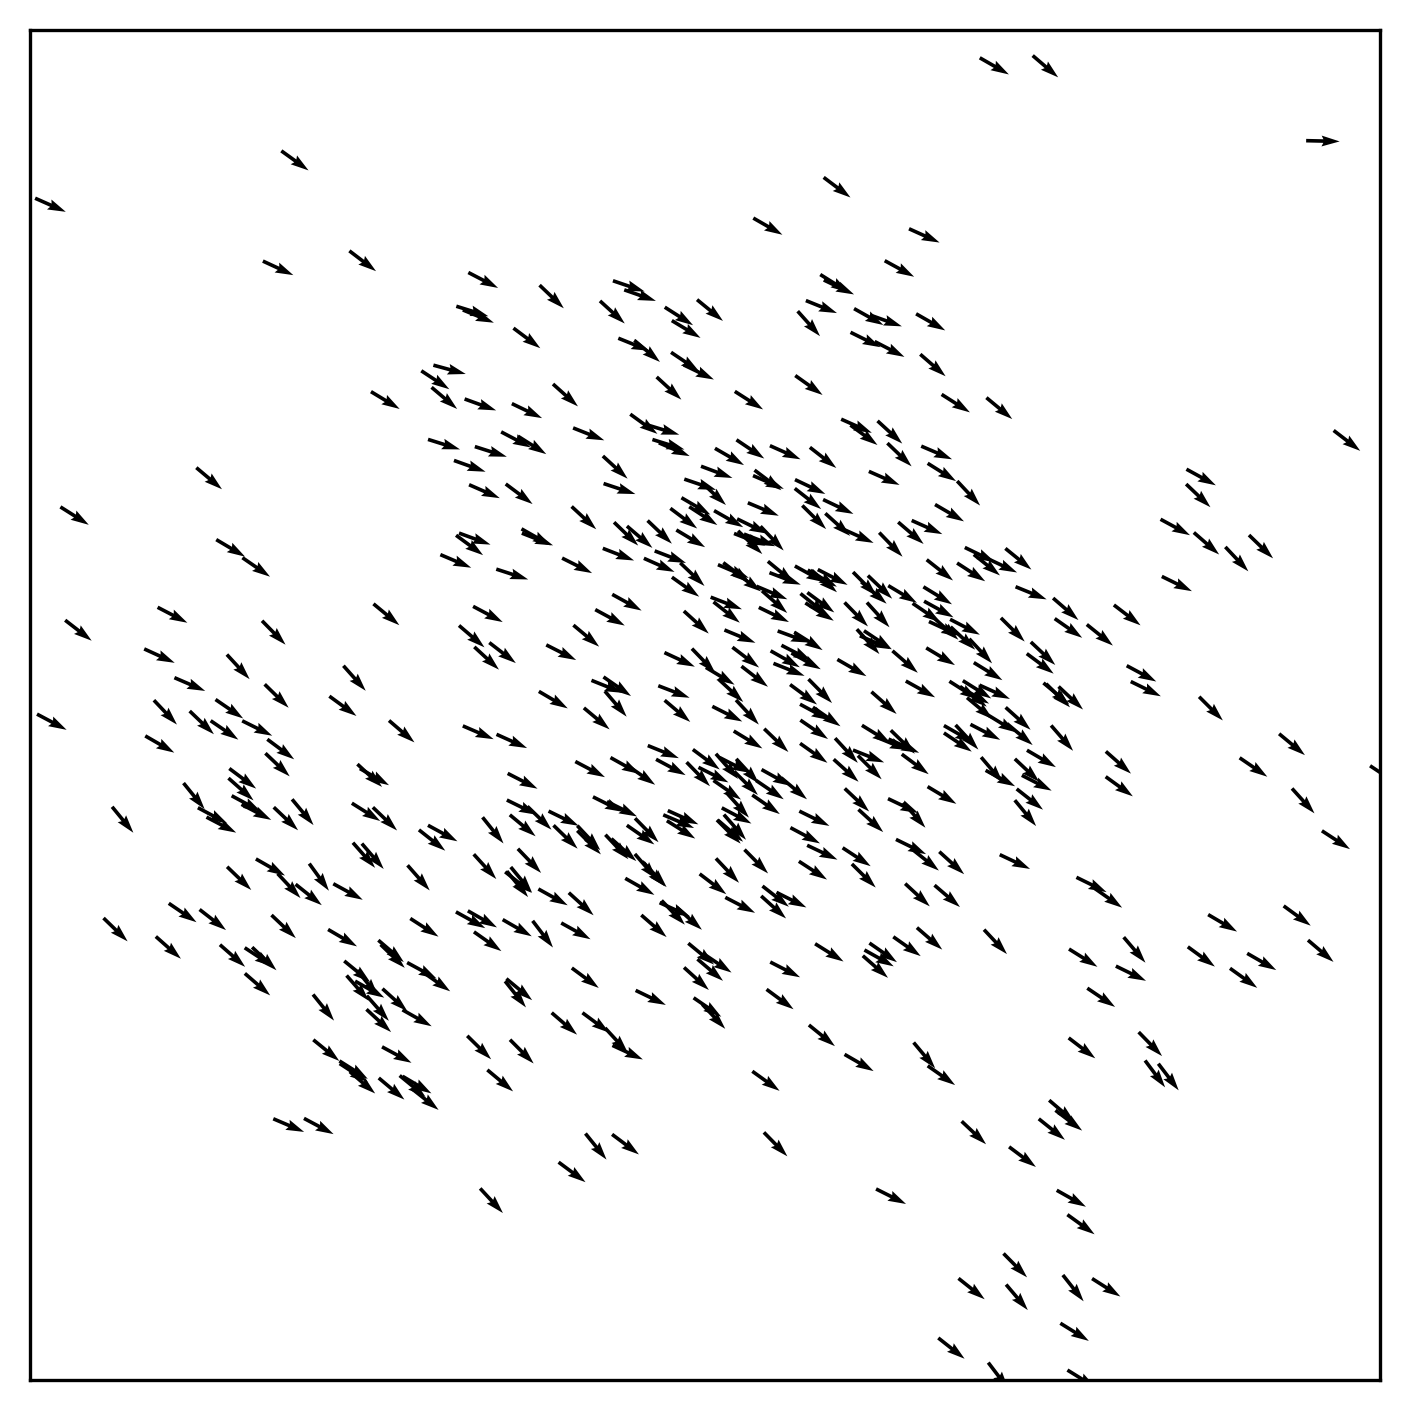
\includegraphics[width=\linewidth]{images/vicsek/VicsekLater.png}
    \end{subfigure}
    \caption{The evolution of the Vicsek model over time. 
    The agents start out moving in random directions but quickly align themselves with each other.}
    \label{fig:VicsekTimeEvolution}
\end{figure}
\begin{align}
    \left\langle\theta(t)\right\rangle _R &= \tan ^{-1}\left(\frac{\langle \sin(\theta)\rangle _R}{\langle \cos(\theta)\rangle _R}\right) \,.
\end{align}
In their paper, Vicsek et al used a uniform distribution to choose the \(\Delta\theta\) for each particle, at each timestep.
They chose a random value from the range [\(-\eta/2, \eta/2\)] to perturb the direction of the particle, which represents the noise
of the system. The magnitude of the noise may be controlled by adjusting the \(\eta\) parameter. In their paper,
an order parameter \(\varphi(t)\) was introduced to measure the alignment of the trajectories of the particles. 
It represents the normalized average velocity of the particles and
may be 
calculated by
\begin{align}
    \varphi(t) &= \frac{1}{Nv}\left|\sum_{i=1}^{N}\mathbf{v}_i(t)\right|\,.
\end{align}
\(\varphi\) therefore has a range between 0 (completely disordered motion) and 1 (fully aligned motion).
The paper then goes on to inspect the effects of the various system parameters on this order parameter.
The parameters that can be changed are the number of particles \(N\), the interaction radius \(R\) for aligning with neighbouring
particles, and the strength of the noise \(\eta\). 

\subsection{Vicsek Model Results}

\begin{figure}[tb]
    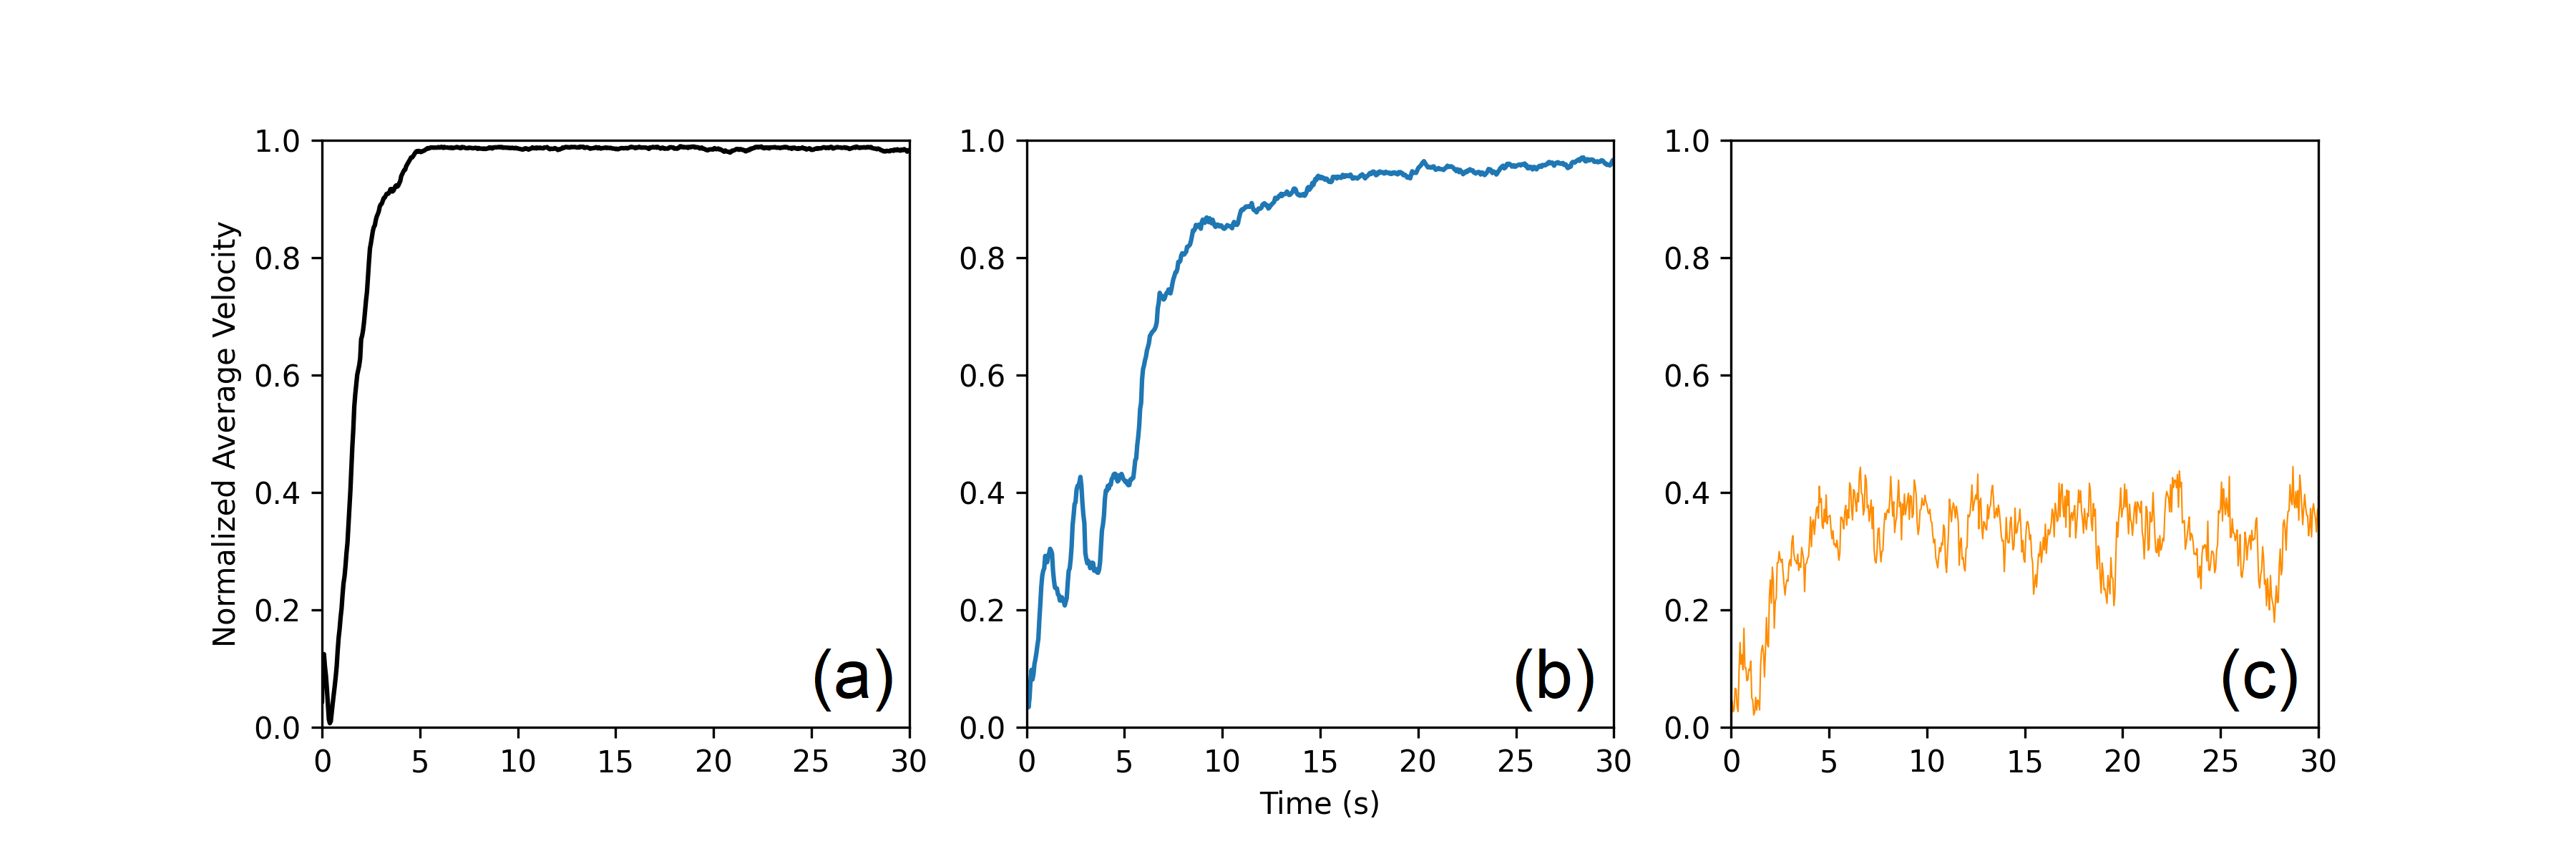
\includegraphics[width=\textwidth]{figures/vicsek/averageVelocities.png}
    \caption{The behaviour of the normalized average velocity \(\varphi\) with time.
    (a) The base case \(N=500, R=1, \eta=0.5\).
    (b) Smaller interaction radius \(R=0.3\).
    (c) Greater magnitude for the noise parameter \(\eta=4\).
    }
    \label{fig:VicsekPhiTime}
\end{figure}


I have produced an investigation into this model and the effects of the various parameters on the order parameter \(\varphi\).
The results can be seen in Fig. \ref{fig:VicsekPhiTime} and Fig. \ref{fig:VicsekPhiEta}. Initially I used the same 
parameters as in the Vicsek paper and measured \(\varphi\) over a period of 30 seconds, which can be seen in Fig. \ref{fig:VicsekPhiTime}a.
The value quickly approached 1 and stayed there for the rest of the simulation. I then reduced the size of the interaction
radius \(R\) to 30\% its initial size. The result is that \(\varphi\) took longer to tend towards the previous value of 1.
Intuitively, this makes sense as fewer interactions between particles would imply taking a longer time to self-align
with each other. Next, I returned \(R\) back to its initial value and increased the noise magnitude \(\eta\) eightfold
from \(\eta = 0.5\) to 4. This had the effect of reducing the value that \(\varphi\) tended towards, as well as cause instability
in the value as it jumped up and down. It would be interesting to investigate the size of this fluctuation in a later study but
at the time I was only interested in the value the average tended towards as this is what was conducted in the paper by Vicsek et al.

Fig. \ref{fig:VicsekPhiEta} is the data I received after measuring the average value of \(\varphi\) for various 
noise magnitudes \(\eta\) and particle numbers \(N\). The figure itself visually matches a similar figure produced in the paper \cite{vicsek1995novel},
which measured the same parameters with the same conditions. I can therefore say I have successfully reproduced their results
and can make similar conclusions. In the paper they note that the order parameter \(\varphi\) is similar to an order parameter
for some equilibrium systems close to their melting point.
\begin{figure}[tb]
    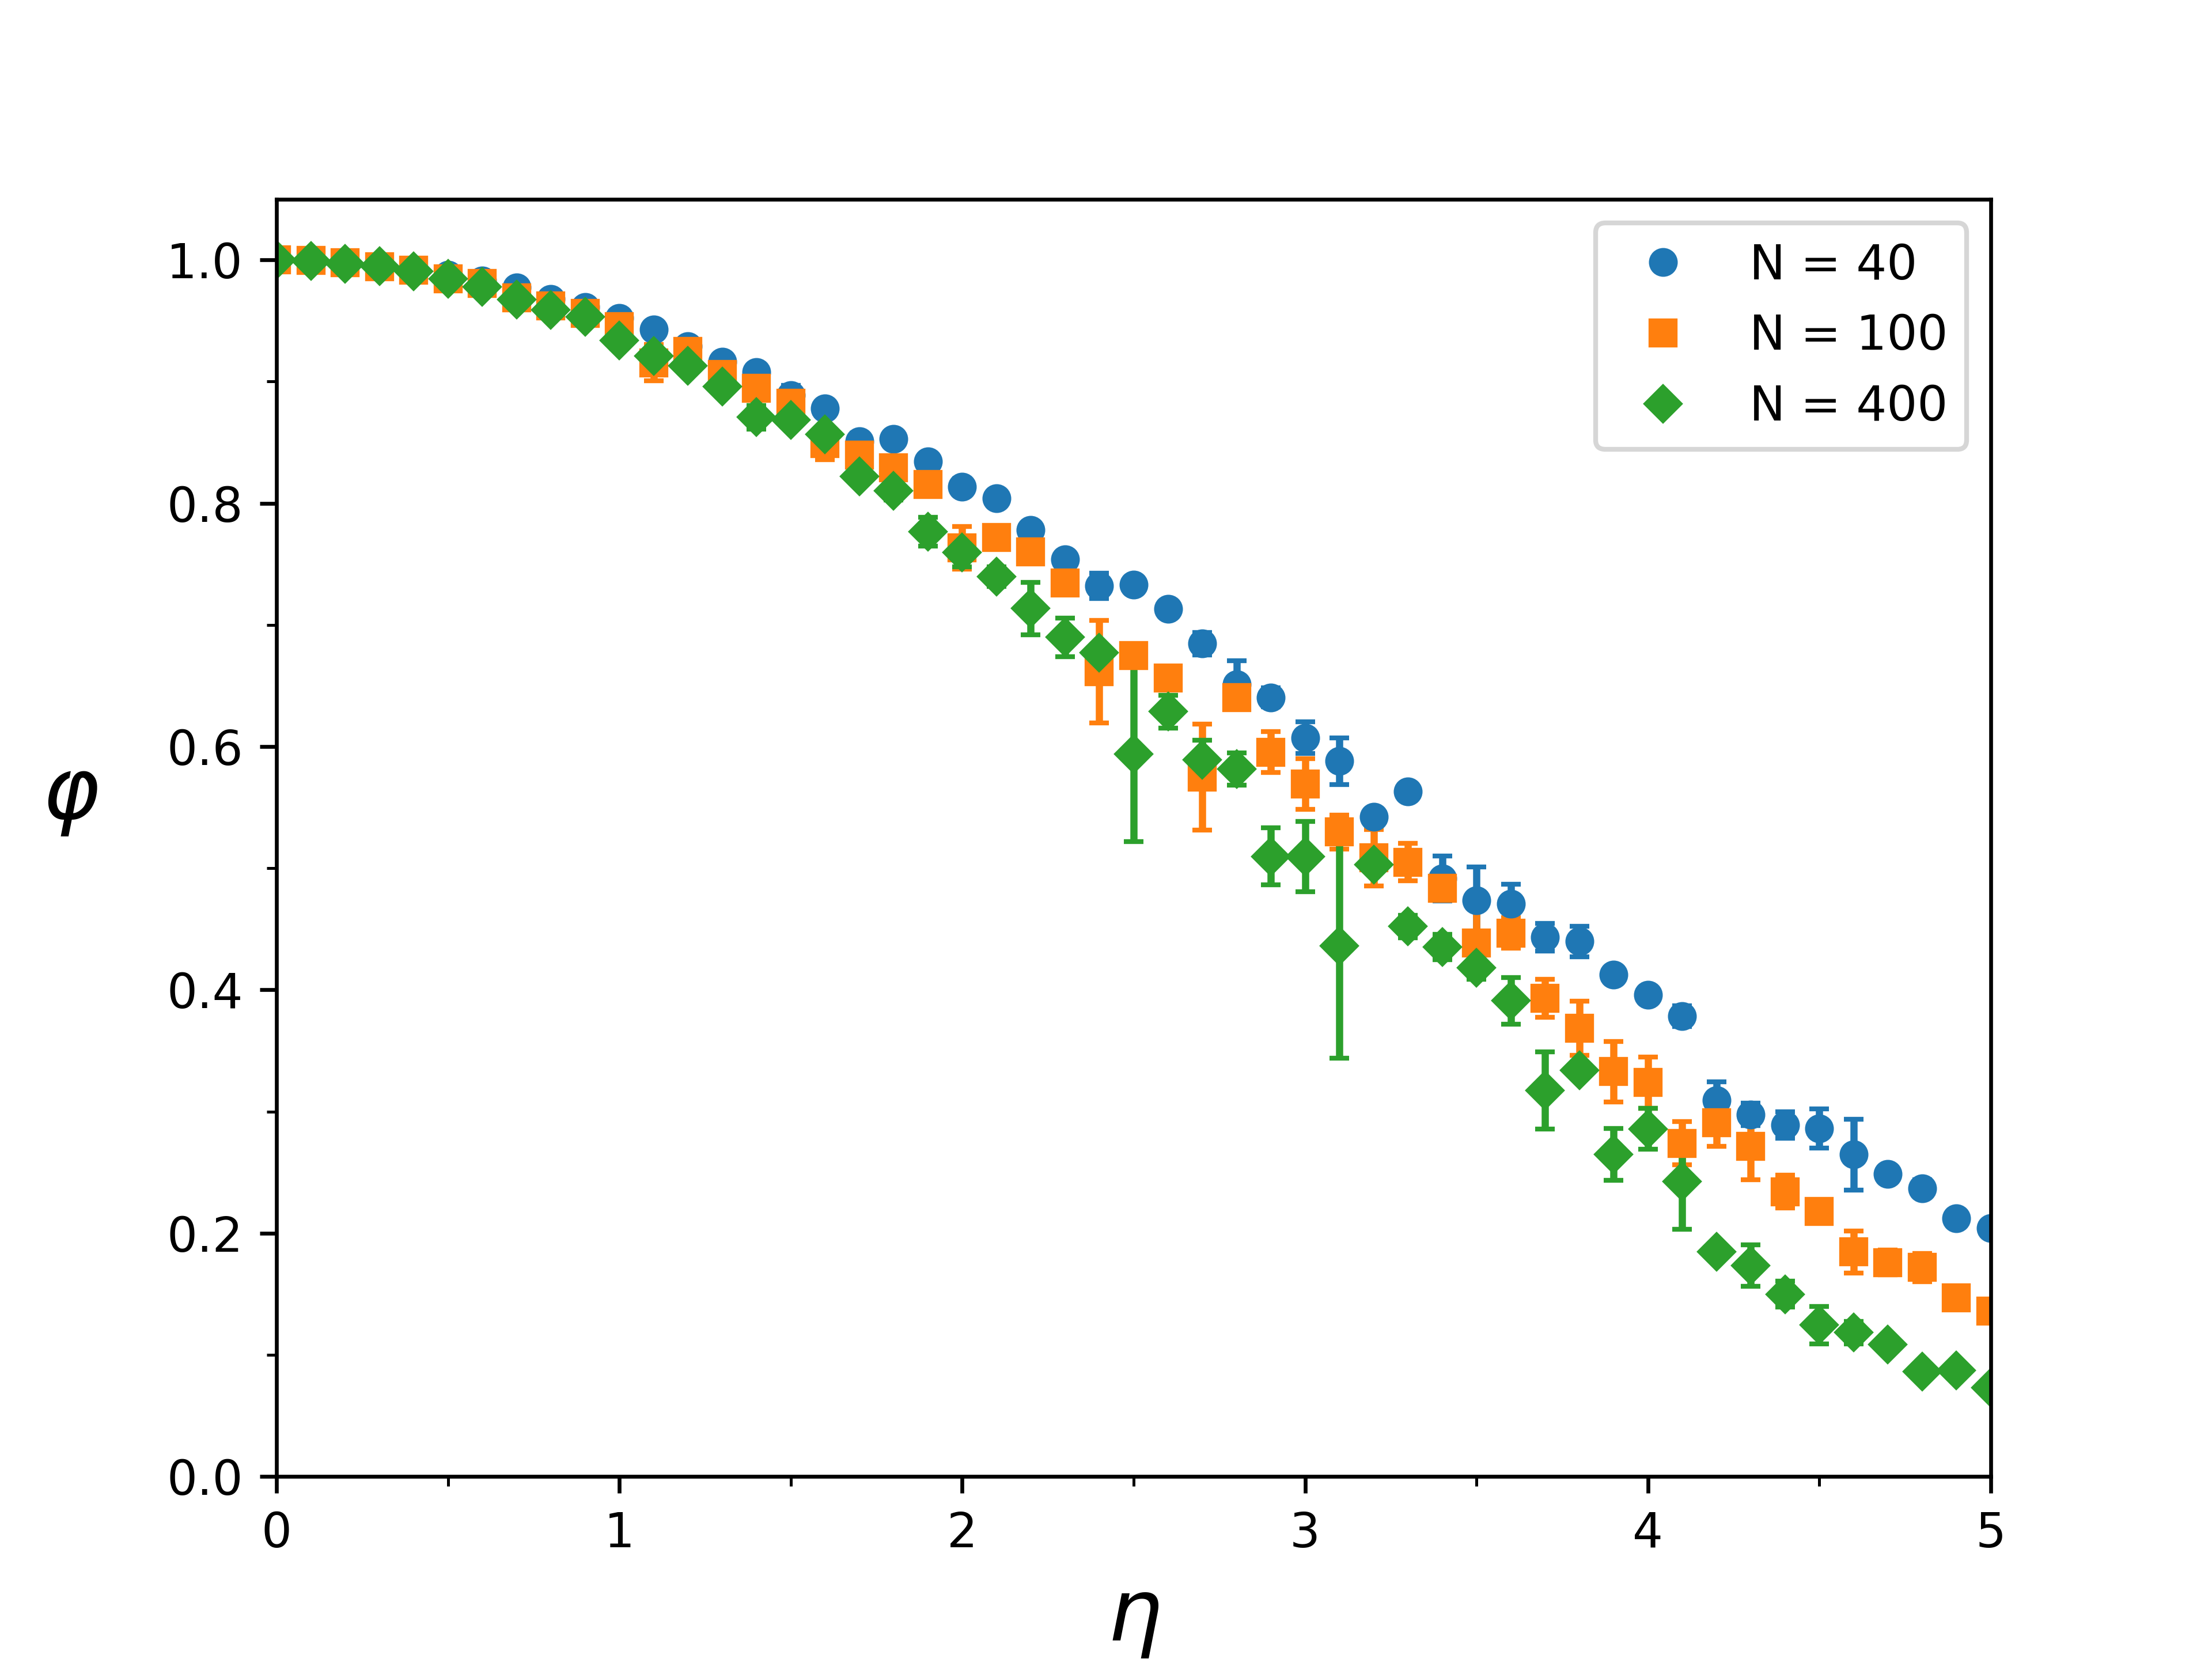
\includegraphics[width=0.5\textwidth]{figures/vicsek/variationOfMeanVelocityWithNoise.png}
    \caption{The average value of \(\varphi\) after \(t=300\) seconds, for varying noise magnitude \(\eta\) 
    and particle number \(N\).}
    \label{fig:VicsekPhiEta}
\end{figure}

\section{Chase \& Escape Model}
Whilst the previous model was interesting, I preferred to investigate systems that are more natural and less abstract. 
I also was interested in studying areas in collective motion that aren't investigated as often. For these reasons I
decided to look into two species systems, where one species' goal is to hunt the other. This type of system appears very
frequently in nature, with groups of predators hunting down herds of prey. 

When focusing on this area, I encountered a paper authored by Janosov, with Vicsek et al as co-authors \cite{janosov2017group}.
In this paper, they discuss a system in which a group of 'chasers' are trying to catch another group of 'escapers'. 
The chasers aren't as fast as the escapers so they need to use cooperative behaviours and smart tactics to successfully
catch the escapers. Instead of using fixed velocities, there are now simulated 'forces' which can accelerate the individual
species agents up to a maximum top speed.

\subsection{Chase \& Escape Model Setup}
There are now \(N_c\) chasers and \(N_e\) escapers in a system, with top speeds \(v_{max, c}\) and \(v_{max, e}\) but 
a similar top acceleration \(a_{max}\). 
The position and velocity of the i\(^{th}\) chaser are denoted by \(\mathbf{x}_{c,i}\) and \(\mathbf{v}_{c,i}\) respectively.
Similarly, \(\mathbf{x}_{e,j}\) and \(\mathbf{v}_{e,j}\) denote the position and velocity of the j\(^{th}\) escaper.
An escaper is 'caught' if the distance between it and the closest chaser decreases below a specified capture distance \(r_{cd}\).
The simulation will end once all escapers are caught.
\subsubsection{General rules}

The first difference to the previous model 
is that the system now takes place within a finite circular field of radius \(r_a\), with the origin of our coordinate
space at the center. 
The author of the paper stated that this was chosen to remove edge-effects as much as possible.
The field itself is surrounded by a soft wall \cite{han2006soft} which repulses the species towards the center:
\begin{align}
    \mathbf{v}_i^a &= s(x_i, r_a, r_{wall})\cdot \left(v_{max,k} \, \frac{\mathbf{x}_{i}}{x_i} + \mathbf{v}_i\right)
    ,\,\,\, (k = c, e)
\end{align}
where
\begin{equation}
    s(x_i, r_a, r_{wall}) = \begin{cases}
        0 & \text{if } x_i \le r_a\\
        -\sin^2\left(\frac{\pi}{2 \,r_{wall}} (x_i - r_a)    \right) & \text{if } r_a \le x_i \le r_a + r_{wall} \\
        -1 & \text{if } x_i \ge r_a + r_{wall}
    \end{cases}
\end{equation}
with \(r_{wall}\) the width of the soft wall and \(x_i = |\mathbf{x}_i|\).

Within each species there is also a repulsive force applied between the individual units in order to prevent collisions:
\begin{align}
    v_{k, i}^{coll} &= v_{max, k}\, \hat{\mathcal{N}}\left[  \sum_{j=1}^{N_k} \frac{r_{cd} - d_{ij}}{d_{ij}}\,
    \mathbf{d}_{ij} \, \Theta(r_{cd} - d_{ij}) \right] \\
    \mathbf{d}_{ij} &= \mathbf{x}_{k, i}\, - \,\mathbf{x}_{k, j}\,,\,\, \, \,\,d_{ij} = |\mathbf{d}_{ij}|\,\,\, \, \,(k = c, e)
\end{align}
where \(\Theta\) is the Heaviside step function and \(\hat{\mathcal{N}}\) is a vector normalization operator.

\subsubsection{Chasers}
Chasers will chase the closest escaper whilst working together with other chasers to encircle their prey.
The chasing force is attractive between the chaser and its target and is given by
\begin{align}
    \mathbf{v}_{c, i}^{ch} &= v_{max, c} \, \hat{\mathcal{N}} \left[ 
        \frac{\mathbf{x}_e - \mathbf{x}_{c,i}}{|\mathbf{x}_e - \mathbf{x}_{c,i}|} 
        + C_f' \frac{\mathbf{v}_e - \mathbf{v}_{c,i}}{\,|\mathbf{v}_e - \mathbf{v}_{c,i}|^2}
    \right]
\end{align}
where \(C_f'\) is the coefficient for a velocity alignment term which takes precedence at small distances.

Chasers also try to predict the path of the escapers and intercept them. Instead of aiming for the target position 
\(\mathbf{x}_e\) they instead head towards the point \(\mathbf{x}_e' = \mathbf{x}_e + \mathbf{v}_e\cdot\tau_{pred}\) 
which lies along the current trajectory of the escaper. \(\tau_{pred}\) is how far into the future the chaser will predict the
escaper to continue on its trajectory. If the chaser can intercept the escaper along its trajectory before this point,
it should instead head to the interception point. \(\mathbf{x}_e'\) is therefore the solution to the equation
\begin{align}
    \mathbf{x}_e' &= \mathbf{x}_e + \mathbf{v}_e\,\cdot\,\text{min}\left[ 
        \frac{\mathbf{x}_e' - \mathbf{x}_c}{|\mathbf{v}_c|}, \tau_{pred}
    \right]\,.
\end{align} 

Finally, chasers have an interaction force applied between them. This is to simulate cooperative behaviour. If there was
no cooperation, the chasers will all lag behind the escapers with no chance of catching them. Janosov et al modelled 
this as a repulsive force between the chasers in order to keep them spread out:
\begin{align}
    \mathbf{v}_{c,i}^{inter} = C_{inter} \, v_{max, c}\, &\hat{\mathcal{N}}\left[ 
        \sum_{j}\left( \frac{r_{inter} - d_{ij}}{d_{ij}} \, \mathbf{d}_{ij} \,+ C_f''
        \frac{\mathbf{v}_{c, j} - \mathbf{v}_{c, i}}{d_{ij}^2} \right)
    \right] \\
    \mathbf{d}_{ij} &= \mathbf{x}_{c, i} - \mathbf{x}_{c, j}\,, \quad\quad d_{ij} = |\mathbf{d}_{ij}|
\end{align}
where \(r_{inter}\) is the characteristic length of this repulsion whilst \(C_f''\) is the coefficient of a velocity alignment term.
\(C_{inter}\) is the interaction coefficient which determines the strength of the interaction between chasers with 
\(C_{inter}=1\) representing a force of equivalent magnitude to the chasing force. 

The final force on the i\(^{th}\) chaser is the sum of the general and chaser specific terms
\begin{equation}
    \mathbf{f}_{c, i} = \mathbf{v}_i^a + \mathbf{v}_{c, i}^{coll} + \mathbf{v}_{c, i}^{ch} + \mathbf{v}_{c,i}^{inter}
\end{equation}

\subsubsection{Escapers}
For the model in the paper, each escaper has a radius \(r_{sense}\) around them in which they can detect any chasers.
When an escaper detects chasers around them, there will be a repulsive force between each chaser and the escaper applied to the
escaper proportional to the inverse squared distance between. This represents a prey species prioritising closer predators
when choosing which direction to escape. The term is given by 
\begin{align}
    \mathbf{v}_{e, i}^{esc} &= v_{max, e}\, \hat{\mathcal{N}}\left[ 
        \sum_{j}\left(  \frac{\mathbf{x}_{e, i} - \mathbf{x}_{c, j}}{\;|\mathbf{x}_{e, i} - \mathbf{x}_{c, j}|^2} 
        - C_f''' \frac{\mathbf{v}_{e, i} - \mathbf{v}_{c, j}}{\;|\mathbf{x}_{e, i} - \mathbf{x}_{c, j}|^2}         \right)
        \Theta(r_{sense} - |\mathbf{x}_{e, i} - \mathbf{x}_{c, j}|)
        \right]\,.
\end{align}
This form of escaping alone is quite simple and basic. Janosov introduced erratic escaping into their as a means to replicate
the erratic movements a prey species might make whilst fleeing for its life. They introduce zigzagging into the escapers'
behaviour as a way to represent more realistic behaviours seen in nature.
Each escaper has a panic parameter \(p_{panic}\) which is an exponential function of the minimum distance to the closet chaser
\(d_{min}\). It is calculated by 
\begin{equation}
    p_{panic} = \begin{cases}
        \frac{1}{e-1}\,\left[e^{1 - d_{min}/r_{sense}} - 1\right] & d_{min} \le r_{sense}\\
        0 & d_{min} \ge r_{sense}
    \end{cases}
\end{equation}
therefore \(p_{panic}\) ranges from 0 when it does not detect any chasers to 1 when the closest chaser is at the same position as the escaper.
Once the panic parameter meets the threshold \(p_{panic} > p_{thresh}\), and assuming there's at least a reasonable distance \(r_{zigzag}\) from the
wall (\(r_a - |\mathbf{x}_e| > r_{zigzag}\)) the escaper will begin zigzagging in order to avoid its pursuers.
The direction angle is chosen randomly from the range [0, \(2\pi\)] and the magnitude of the zigzag component 
\(|\mathbf{v}_{e, i}^{zigzag}| = v_{max, e}\). The length of time spent on  a single zigzag length
is also a random parameter with a lower bound \(r_{zigzag}/v_{max, e}\) and upper bound \(r_{a}/v_{max, e}\).

To account for possibly of an escaper trying to flee outside the wall and reducing its speed as a result, Janosov adds  
a condition where the radial part of the velocity decreases the closer to the wall the escaper gets. 
\begin{equation}
    \mathbf{v}_e^{final} = \mathbf{v}_e - C_{wall} \frac{\mathbf{x}_e}{|\mathbf{x}_e|}
    \left(\frac{\mathbf{x}_e}{|\mathbf{x}_e|} \cdot \mathbf{v}_e \right) = \hat{\mathbf{W}}\mathbf{v}_e
\end{equation}
where
\begin{equation}
    C_{wall} = \begin{cases}
        1 & r_a - |\mathbf{x}_e| < 2 \, r_{wall} \\
        \cos^2\left(\frac{\pi}{2\,r_{zigzag}}(|\mathbf{x}_e| - r_a +2 r_{wall}) \right) & r_a - |\mathbf{x}_e| < 2\,r_{wall} + r_{zigzag} \\
        0 & \text{otherwise.}
    \end{cases}
\end{equation}

By itself, this would cause the escaper to get stuck at the wall once it reaches there. A condition is therefore introduced:
if the escaper is close to wall (\(C_{wall} > 0.5\)) and it is capable of slipping past the two closest chasers and return to the center
of the field, it will do so. To calculate if it is possible, first determine the direction vector pointing along the line 
which evenly separates the two chasers
\begin{equation}
    \mathbf{e} = \frac{(\mathbf{x}_{c, 1} - \mathbf{x}_{e}) + (\mathbf{x}_{c, 2} - \mathbf{x}_{e})}{|(\mathbf{x}_{c, 1} - \mathbf{x}_{e}) + (\mathbf{x}_{c, 2} - \mathbf{x}_{e})|}\,.
\end{equation}
Then calculate the two points at which the two chasers will perpendicularly bisect the line 
\begin{equation}
    \quad\mathbf{x}_{p, k} = \mathbf{x}_{e} + \mathbf{e} \, [\mathbf{e} \cdot (\mathbf{x}_{c, k} - \mathbf{x}_e)]\quad(k = 1,2).
\end{equation}
The minimum times for the escaper to reach those points are given by
\begin{equation}
    \tau_{e, k} = \frac{|\mathbf{x}_{p, k} - \mathbf{x}_e|}{v_{max, e}}
\end{equation}
whilst the times for the chasers are
\begin{equation}
    \tau_{c, k} = \frac{|\mathbf{x}_{p, k} - \mathbf{x}_{c, k}| - r_{cd}}{v_{max, c}}\,.
\end{equation}
If \(\tau_{e, k} < \tau_{c, k}\) for both \(k = 1 \) and 2, the escaper can successfully pass between the two chasers and 
return to the center. Otherwise, it stays at the wall.

The final force on the i\(^{th}\) escaper is the sum of the general terms and either the basic escaping force or the zigzag
force, transformed by the \(\hat{\mathbf{W}}\) operator in Eq. 16.

\begin{equation}
    \mathbf{f}_{e, i} = \hat{\mathbf{W}}(\mathbf{v}_i^a + \mathbf{v}_{e, i}^{coll} + (\mathbf{v}_{e, i}^{esc} \textbf{ or } \mathbf{v}_{e, i}^{zigzag}))
\end{equation}



\begin{figure}[tb]
    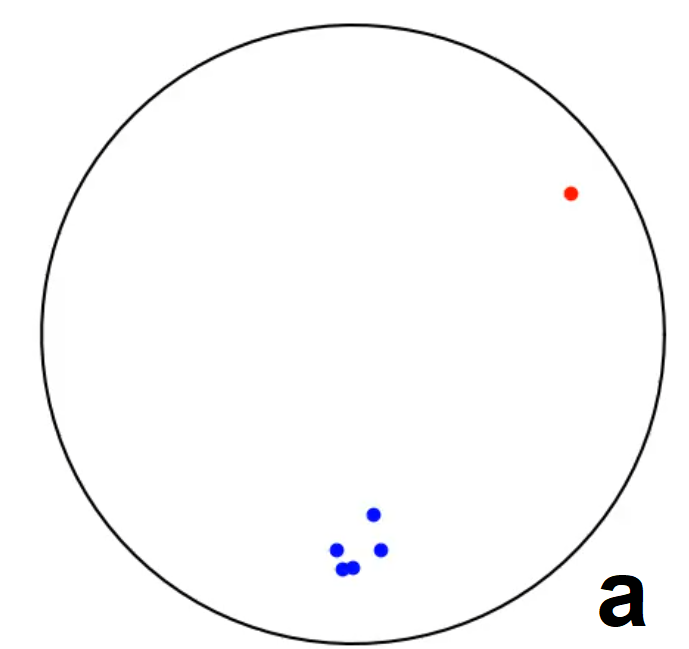
\includegraphics[width=\threeImageSpacing]{images/chaseescape/0.png}
    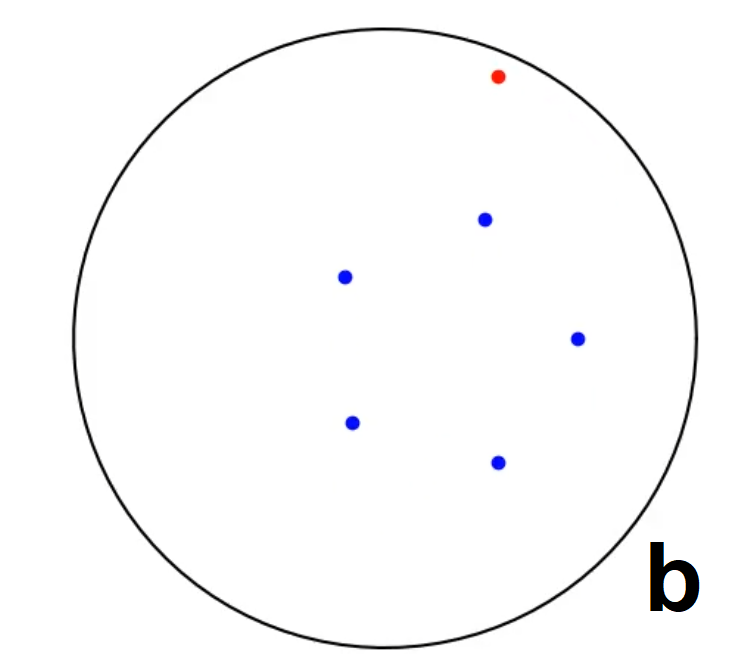
\includegraphics[width=\threeImageSpacing]{images/chaseescape/1.png}
    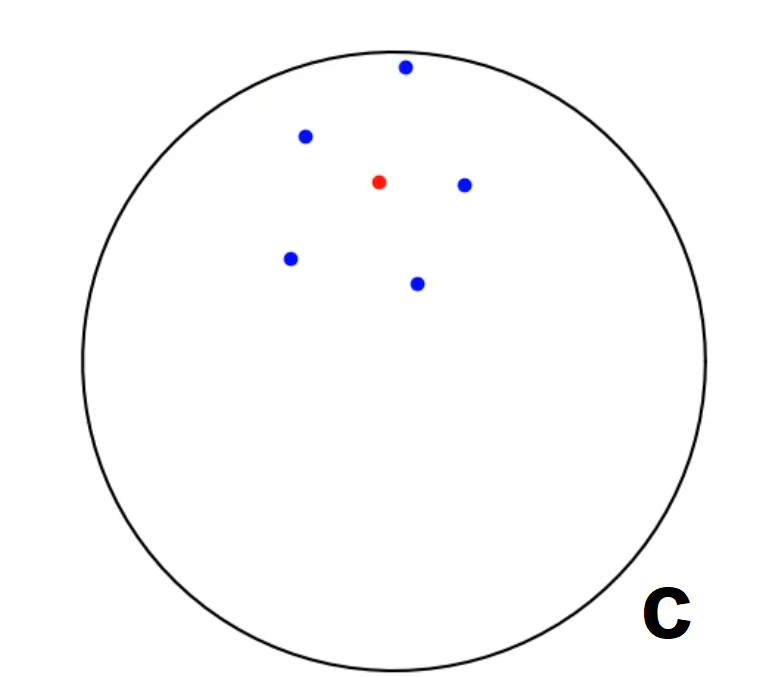
\includegraphics[width=\threeImageSpacing]{images/chaseescape/2.png}
    \caption{The time evolution of the chase \& escape model. The chasers (blue) hunt down the escaper (red) and encircle
    it before quickly catching it.}
    \label{fig:chaseescape}
\end{figure}
\newpage
\begin{table}[tb]
    \begin{center}
    \setlength\extrarowheight{-3pt}
    \begin{tabularx}{\textwidth}{X p{3cm} p{3cm}}
        \hline\hline
        Parameter description & Symbol & Value \\
        \hline
        Maximum Acceleration of chaser/escaper & \(a_{max}\) & 6 \\
        Radius of circular field& \(r_a\) & 150 \\
        Width of enclosing wall  & \(r_{wall}\) & 5 \\
        Minimum distance for capture & \(r_{cd}\) & 1 \\
        Friction coefficient in chasing term & \(C_f'\) & 1.1 \\
        Friction coefficient in chaser velocity alignment & \(C_f''\) & 1.1 \\
        Friction coefficient in escaping term & \(C_f'''\) & 1.1 \\
        Maximum time allowed for simulation to run & \(T_{max}\) & 5000 \\
        \hline
        Number of chasers & \(n_c\) & 1-5 \\
        Chaser top speed & \(v_{max, c}\) & 6 \\
        Upper limit on chaser's prediction time frame & \(\tau_{pred}\) & 6 \\
        Strength of interaction between chasers & \(C_{inter}\) & 0.4 \\
        Characteristic interaction distance between chasers & \(r_{inter}\) & 100 \\
        \hline
        Number of escapers & \(n_e\) & 1-5 \\
        Escaper top speed & \(v_{max, e}\) & 8 \\
        Escaper panic threshold & \(p_{thresh}\) & 0.7 \\
        Escaper's range of vision & \(r_{sense}\) & 150 \\
        Minimum distance required for zigzag & \(r_{zigzag}\) & 40 \\
        \hline        
    \end{tabularx}
    \caption{List of parameters for chase \& escape model, with their symbol and the values used in testing.}
    \label{tab:ChaseEscape}
    \end{center}
\end{table}
\subsection{Chase \& Escape Testing Method}
With this model I will be investigating the time required for the chasers to fully capture the escapers. In case the
escaper group can successfully evade the chasers indefinitely, I have a fixed limit \(T_{max}\) on the 
time each simulation can run for. All the model parameters are displayed above in TABLE \ref{tab:ChaseEscape}.
The parameters I chose to vary and investigate the results of are the sizes of the two groups, \(n_c\) and \(n_e\). 
I investigated group sizes in the range of 1-5 for both chasers and escapers. 
Future work could investigate a wider range of values for these two, or look at altering any of the other model parameters.

For a given set of \((n_c,n_e)\), I run the simulation and record the time \(T\) it takes to complete. I then repeat the
simulation several more times in order to reduce the effect of random nature on the average. A higher number of runs 
would correlate with a reduction in this random uncertainty. 




\begin{figure}[t]
    \includegraphics[width=0.8\linewidth]{figures/chaseescape/data.png}
    \caption{A heatmap of the average time each simulation lasts, as a fraction of the maximum simulation time \(T_{max}\)}
    \label{fig:chaseescapedata}
\end{figure}
\subsection{Chase \& Escape Model Results}
The data I have collected is displayed above in Fig. \ref{fig:chaseescapedata} as a heatmap of the average simulation
times. For the case of 1 chaser, it cannot catch up to any of the escapers due to its slower speed so the simulation time
\(T\) is equivalent to the maximum time allowed \(T_{max}\). It is apparent that without cooperation from fellow chasers,
the lone chaser would never catch anything.

For the scenarios invloving 2 chasers, the results are mostly the same at face value. Two chasers are not enough to block
every possible escape route in most situations. It is possible for an escaper to be caught however if the chasers are in
the perfect position to pin the escaper against the wall, although the precise positions and velocities required leave the
probability of an escaper being caught quite low. On average, only 1 escaper is caught before \(T_{max}\). Interestingly
there was one simulation with \((n_c,n_e) = (2,4)\) where all the escapers were caught. Given that most simulations
with \(n_c=2\) only had 1 escaper being caught, I conclude that this must be an extremely unlikely event.

For \(n_c \ge 3\), the chasers could now encircle and trap their prey. Looking at the data for \(n_e=1\), increasing
the number of chasers encircling an escaper past \(n_c=3\) does not reward much benefit in reducing the time to catch.
I can therefore predict that there is a fixed lower bound on \(T\)  that scales proportionally with the number of escapers \(n_e\). 
This does not take into account chasers only target the closest escaper, so there might not be 3 chasers targeting a specific escaper.

For larger values of \(n_c\) and \(n_e\), the data behaves predictably. Increasing the number of escapers increases
the simulation time, whilst increasing the number of chasers shortens it. Interestingly, these two aren't equivalent in magnitude;
increasing both group sizes by an equivalent amount will increase the simulation time. A possible explanation is that
it takes multiple chasers to capture an escaper, so increasing the chaser population by only 1 chaser would not be enough
to account for an additional escaper. The exact number of additional chasers required to "match" an additional escaper
could be a topic for future work. 

\section{Predator-Prey Model}
After I had constructed the previous model, I understood that it was effective for the simple yet complex chasing scenarios
that predator species perform with their prey in nature. Thinking along those lines, I decided that my next step was to
investigate a model that incorporates more aspects of nature. I also felt confident enough with my knowledge of creating models
by this point to create my own model.

This model, like the chase \& escape model by Janosov \cite{janosov2017group}, is a two species model with a "predator" group
trying to catch their "prey". There are several differences however. Firstly, my prey species have a "nest" area that they can
safely be without risk of being captured by the predators. This is a direct parallel to the nests and habitats some
animals in nature posses, such as the nests of a flock of birds or a burrow for rabbits. Secondly, I have given the
prey species an objective to collect food. They must collect a certain amount of food in order to survive or else they
"starve". 

The two species in my model therefore have conflicting objectives. The predators must hunt the prey to extinction, whilst the prey
species must collect enough food to survive without all being caught.  


\subsection{Predator-Prey Model Setup}
I chose to use a 2D box setup of length \(2L\) as my environment, as it is simple to implement in practice.
The origin is the center of the box.
The nest for the prey is placed at a random position within the box, and \(n_{prey}\) prey with positions \(\left\{\mathbf{x}_i^{prey}\right\}_{i=1}^{n_{prey}}\)
are placed randomly within radius \(r_{nest}\) of the nest. The \(n_{pred}\) predators start out together, 
placed at a random point \(\mathbf{x}_j^{pred}\) within the box
excluding the circular region representing the nest of the prey.

The food is spawned in groups, with each group placed at a random point in the box not including the nest area. There are
\(n_{\text{fg}}\) food groups and \(n_{\text{fopg}}\) food objects per group. The food objects are placed randomly within
\(r_{food}\) of the food group center location.

There is a maximum acceleration \(a_{max}\) for both species, with different top speeds \(v^{prey}\) and 
\(v^{pred}\) respectively.

\subsubsection{General rules}
The walls of the environment are hard walls. I chose these over periodic boundaries to prevent indefinite chases.
In order to implement these hard walls, I consider the coordinates and velocity of both the predators and prey at each timestep.
I check the future position of a subject against the wall boundaries (\(x=\pm L,y=\pm L\)) and if it
 were to move past a wall, I zero the velocity component responsible for crossing the bondary and rescale
the velocity vector accordingly. This has the effect of making the subject move parallel to the wall at it's previous speed
instead of colliding head first into it.

I have also chosen to model fatigue in my predators and prey. I express this by modelling the top speed of the species
as a variable that decays exponentially over time

\begin{align}
    v^k &= v_0^k \cdot e^{-\frac{t}{\tau_k}}, \hspace{1cm} (k= \text{pred, prey})
\end{align}
where \(\tau_{pred}\) and \(\tau_{prey}\) are the decay times for each sepcies respectively.

\subsubsection{Predators}
Like the previous model, a predator will hunt down its target using Eq. 9. However, in contrast to the cooperative nature
of those chasers, the predators of this model are simpler and instead hunt seperately. In the beginning of the simulation,
iterate over each predator and set its target to the closest prey that isn't also being targeted. When a prey is captured,
the responsible predator will again try to target a prey not already being targeted, otherwise it just hunts the closest.
My reason for setting the behaviour of the predator this way is because the predators have to catch all the prey before they
collect the food and return to the safety of their nest. This strategy could be considered more efficient for quickly
eliminating the prey species, and the predators start out faster in this model so cooperation between predators is not important
for ensuring capture.
\begin{table}[t]
\begin{center}
    \setlength\extrarowheight{-3pt}
    \begin{tabularx}{\textwidth}{X p{3cm} p{3cm}}
        \hline\hline
        Parameter description & Symbol & Value \\
        \hline
        Half length of side of box & L & 100 \\
        Prey spawn radius around nest & \(r_{nest}\) & 10 \\
        Number of groups of food & \(n_{fg}\) & 3 \\
        Number of food objects per group & \(n_{fopg}\) & 4 \\
        \hline
        Number of predators & \(n_{pred}\) & 1-5 \\
        Predator initial speed & \(v_0^{pred}\) & 3-4 \\
        Predator fatigue time & \(\tau_{pred}\) & 1500 \\
        \hline
        Number of prey & \(n_{prey}\) & 1-5 \\
        Prey initial speed & \(v_0^{prey}\) & 3 \\
        Prey fatigue time & \(\tau_{prey}\) & 2000\\
        \hline
    \end{tabularx}
    \caption{The list of parameters and the values used for the predator-prey model.}
    \label{tab:predprey}
\end{center}

\end{table}
\subsubsection{Prey}
Like the predators, each prey is assigned a unique food object it must aquire. It will attempt to collect the food the same
way a predator hunts its prey

\begin{align}
    \mathbf{v}_i^{prey,food} &= v^{prey} \cdot \frac{\mathbf{x}_i^{food} - \mathbf{x}_i^{prey}}{|\mathbf{x}_i^{food} - \mathbf{x}_i^{prey}|}
\end{align}
where \(\mathbf{x}_i^{food}\) is the position of the food being targeted by the i\(^{th}\) prey.

Prey also fear and attempt to move away from predators the same way escapers from the previous model flee from catchers, using
Eq. 14. 



\subsection{Predator-Prey Model Testing}
With this model I will investigating the two possibles outcomes, prey victory or predator, and the effect the initial
set of parameters have on the outcome. The parameters I will be varying are \(n_{prey}\), \(n_{pred}\), 
and \(v_0^{pred}\). I am investigating the effects of population variation, as well as how the speed of the predator 
affects the outcome.







\subsection{Predator-Prey Model Results}




\begin{figure}[htbp]
    \includegraphics[width=0.87\linewidth]{figures/predatorprey/ExtinctionTime.png}
    \includegraphics[width=0.8\linewidth]{figures/predatorprey/SpeedExtinction.png}
    \caption{(a) A heatmap of the extinction time for the prey species with variation of both species initial
    population number. For coordinates (5, 1) the prey were always able to collect all the food and hence no data.
    (b) A data plot of the total simulation time when the predators' speed was varied. Green signifies all food was collected
    first while red indicates the prey were all caught.}
    \label{fig:numberpredprey}
\end{figure}

The results can be seen below in Fig. \ref{fig:numberpredprey}. For the first set of experiments, I set \(v_0^{pred}=3.5\).
At this speed, the predators were almost always catching the prey, so I measured how long it took for the prey to be captured.
The heatmap in Fig. \ref{fig:numberpredprey}(a) shows the intuitive understanding that increasing the number predators reduces
this "extinction time" whilst increasing the number of prey raises it. Increasing both populations simultaneously decreases
the extinction time, implying that the predators have an advantage over prey. This only seems to occur for low predator 
numbers with higher number of prey. A possible reason is that going from 1 to 2 predators is a bigger impact than going from
3 to 4 chasers. The number of hunters has doubled while the number of prey has has increase less so, relatively. 
Infact, for \(n_{pred} > n_{prey}\) the extinction time increases, which goes with my hypothesis.

For the second set of experiments I set \(n_{prey}=5, n_{pred} = 3\) and then varied the speed of the predators. The results
can be seen in Fig. \ref{fig:numberpredprey}(b). Starting with the ratio \(v_0^{pred}/v_0^{prey}=1\), I increased the 
predators' speed in small increments and measured the outcome and total time for the simulation. Initially,
the predators and prey were the same speed so the predators could never catch the prey. As the speed was increased, the
average simulation time for the prey victory outcome increased. At a ratio of 1.062, predators started winning occaisionally and
their probability of success increased with speed. Around 1.075 theres a 50/50 chance of either side's win condition occuring.
As predator speed is further increased, probability of predator success increases, with the simulation time for such
outcomes decreasing as well. From the data on the graph I can make several extrapolations. If the predator speed was increased
further onwards, the simulation time would trend down towards zero (the predators are immensely fast and catch the prey almost instantly).
If instead the speed was decreased such that the ratio approached zero, the average simulation time would most likely tend
to the same value as if there was no predators.

How the other parameters affect these data sets would also be interesting to investigate and may be the focus of future studies.


\section{Conclusion}
In conclusion, I have investigated several models in the realm of collective motion and have found interesting data in all of them.
I have highlighted above different ways that I could further study these models, including tweaking more system 
parameters and investigating a broader range for parameters already tested.


\bibliography{references}
\newpage\newpage
\section*{Scientific Summary For General Audience}
Collective motion is the name for the cooperative behaviour that can be observed in nature. 
From a flock of starlings flowing together like water, to a school of fish milling in a vortex, 
and even the movement of microorganisms, the phenomenon of collective motion can be observed. 
But why do these species move in such a complex and ordered way? What is the benefit? 
The goal of this paper is to analyse such systems, by recreating the scientific models of previous researchers 
and building up an understanding of the nature of collective motion. 


\end{document}